\chapter{مقایسه}
در این فصل قصد داریم مقایسه‌ای از سه روش متناسب با جنبه‌های مختلف ارائه دهیم.

\section{مقایسه پیچیدگی زمانی}
روش بر پایه ژنتیک غارب و همکاران \cite{ghareb2016hybrid} پیچدگی زمانی بیشتری نسبت به دو روش دیگر دارد. در این روش در مرحله اول با کمک یک معیار انتخاب ویژگی فیلتر تعدادی از ویژگی‌های مناسب‌تر انتخاب می‌شود و سپس در مرحله بعد یک الگوریتم ژنتیک آن هم با معیار انتخاب ویژگی پوشاننده استفاده می‌شود. در روش برپایه ژنتیک مرحله دوم پیچیدگی زمانی زیادی را دارد؛ چراکه روش‌های ژنتیک و روش‌های پوشاننده روش‌های کندی هستند.
\\

حال باید دو روش دیگر را مقایسه کرد. در روش \lr{IGFSS} آیسال یک بار امتیاز یک معیار جهانی و یک بار امتیاز یک معیار محلی حساب می‌شود. سپس در بدترین حالت دو بار باید لیست ویژگی‌ها را پیمایش کرد؛ یک بار هنگام تشکیل مجموعه ویژگی‌های انتخاب‌شده اولیه و بار دیگر در مرحله بخش شرطی و رساندن تعداد ویژگی‌ها به یک اندازه خاص.\cite{uysal2016improved} در روش \lr{MRDC} لبنی و همکاران یک بار برای تمام ویژگی‌ها معیار تمایزگر نسبی را حساب می‌کنند و سپس نیاز است تا مقدار \lr{MDRC} حساب شود که محاسبه \lr{Correlation} اصلی‌ترین قسمت آن است.\cite{labani2018novel} در این شرایط به نظر می‌رسد که روش \lr{IGFSS} روش سریع‌تری است چرا که لازم نیست تا دو ویژگی نسبت به هم سنجیده شوند و در نتیجه پیچیدگی آن در شرایطی که ابعاد مسئله بسیار بالاست به
$O(|F|^2)$
نمی‌رسد ولی پیچیدگی زمانی \lr{MDRC} از
$O(|F|^2)$
بیشتر است.


\section{مقایسه پیچیدگی حافظه}  
از منظر حافظه‌ي مورد نیاز الگوریتم هم باز روش برپایه ژنتیک به حافظه بیشتری نیاز دارد؛ چراکه در مرحله دوم که قرار است الگوریتم ژنتیک اجرا شود به تعداد اعضای هر نسل باید مجموعه‌ای از ويژگی‌ها نگهداری شود. دو الگوریتم دیگر از نظر حافظه تفاوت چندانی با یکدیگر ندارند.

\section{مقایسه دقت}
در این پروژه پیاده‌سازی‌ای از الگوریتم‌ها تهیه نشده است و در عین حال پیاده‌سازی آماده‌ای هم برای این‌ها در دسترس نبوده است؛ لذا برای مقایسه دقت مستقیما به اعداد مقاله‌ها مراجعه شده است. اما اعداد در مقاله‌ها امکان مقایسه دقیق و عادلانه را به وجود نمی‌آورند. چراکه غارب و همکاران از پیکره‌های عربی استفاده کرده‌اند. آیسول و لبنی و همکاران از تعدادی پیکره استفاده کرده‌اند که برخی از آن‌ها مشترک است ولی با این حال تنظیمات متفاوت که اعمال کرده‌اند باعث می‌شود که همچنان مقایسه عادلانه‌ای را نتوان انجام داد. برای این دو روش نتایج بر روی مجموعه‌داده رویترز را گزارش خواهیم کرد. این مجموعه‌داده هم در دو روش مشترک است و هم آنکه قسمت آموزش و ارزیابی آن توسط خود مجموعه‌داده تعیین شده است. برای روش غارب و همکاران هم تنها یکی از مجموعه‌داده‌ها یعنی الجزیره بررسی می‌شود. در اینجا بنا به محدودیت فقط همین موارد بررسی می‌شوند. برای دیدن سایر نتایج می‌توانید به خود مقالات مراجعه کنید.

\subsection{دقت روش \lr{IGFSS}}
یکی از مشکلاتی که در کار تحقیقاتی اویسال به آن اشاره شده است این است که معیار‌های سنتی به تعداد ویژگی هر کلاس و نسبت ویژگی‌های منفی اهمیت نمی‌دهند. این مورد در تصویر ۴-۱ به خوبی پیدا است. در این تصویر توزیع ویژگی‌ها برای معیار شاخص جینی آورده شده است.

\begin{figure}[!h]
\begin{center}
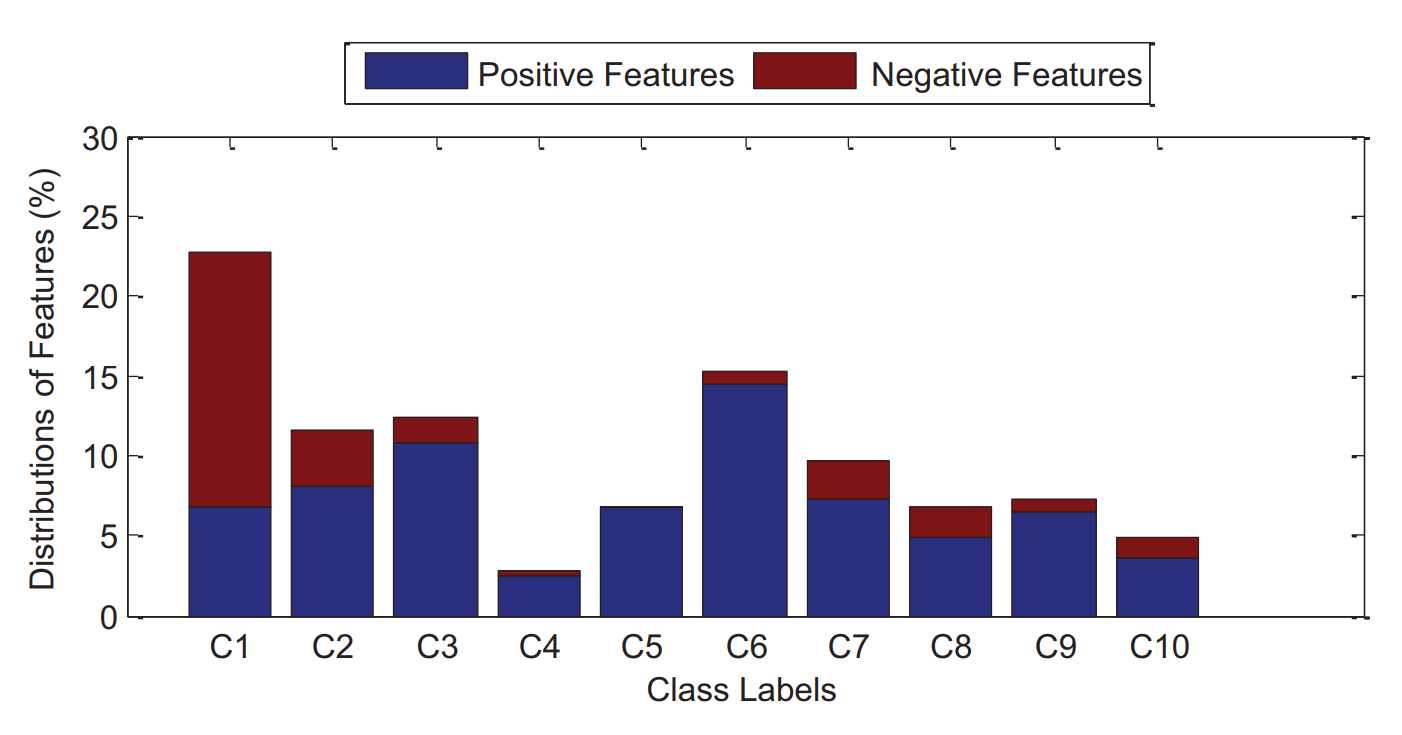
\includegraphics[height=7cm]{IGFSS1.png}
\end{center}
\caption{فراوانی ویژگی‌های انتخاب‌شده نسبت به هر کلاس برای شاخص جینی در روش \lr{IGFSS} \cite{uysal2016improved} }
\end{figure}

در جدول ۴-۱ و ۴-۲ به ترتیب دقت مربوط به روش‌های مختلف انتخاب ویژگی برای دسته‌بند \lr{SVM} و \lr{Naive bayes} بدون استفاده از روش \lr{IGFSS} و با استفاده از آن آورده شده است. با بررسی کلی در می‌یابیم که استفاده از روش پیشنهادی در مقاله منجر به بهبود روش پایه می‌شود اما این بهبود چندان موثر نیست و در هیچ یک از موارد شاهد بیش از ۲ درصد بهبود نیستیم.

\begin{table}
\begin{center}
\caption{معیار $F_1$ برای روش‌های پایه و \lr{IGFSS} برای دسته‌بند \lr{SVM} \cite{uysal2016improved}}
\begin{tabular}{r|r|r|r|r|r|r|r}
\toprule
\textbf{روش} & \textbf{\lr{nfr}} & \textbf{۲۵۰} & \textbf{۳۰۰} & \textbf{۳۵۰} & \textbf{۴۰۰} & \textbf{۴۵۰} & \textbf{۵۰۰}  
\\
\hline
\hline
\lr{IG} & - & ۸۵/۷۵۵ & ۸۶/۰۰۶ & ۸۶/۰۰۶ & ۸۵/۸۶۳ & ۸۶/۰۰۶ & ۸۵/۸۲۷
\\
\lr{IG+IGFSS} & ۰/۶ & ۸۵/۳۶۱ & ۸۶/۴۷۳ & ۸۶/۱۵۰ & ۸۶/۲۹۴ & ۸۶/۱۱۴ & ۸۶/۰۰۶
\\
\lr{GI} & - & ۸۵/۹۳۵ & ۸۵/۹۷۱ & ۸۶/۰۰۶ & ۸۶/۴۰۱ & ۸۶/۰۷۸ & ۸۶/۴۳۷
\\
\lr{GI+IGFSS} & ۰/۳ & 85/648 & 85/791 & 86/329 & 86/437 & 86/760 & 85/935
\\
\lr{DFS} & - & 85/899 & 85/899 & 85/971 & 85/791 & 85/899 & 85/791
\\
\lr{DFS+IGFSS} & ۰/۸ & 85/002 & 86/258 & 86/473 & 86/258 & 86/114 & 85/863
\\
\bottomrule
\end{tabular}
\end{center}
\end{table}

\begin{table}
\begin{center}
\caption{معیار $F_1$ برای روش‌های پایه و \lr{IGFSS} برای دسته‌بند \lr{NB} \cite{uysal2016improved}}
\begin{tabular}{r|r|r|r|r|r|r|r}
\toprule
\textbf{روش} & \textbf{\lr{nfr}} & \textbf{۲۵۰} & \textbf{۳۰۰} & \textbf{۳۵۰} & \textbf{۴۰۰} & \textbf{۴۵۰} & \textbf{۵۰۰}  
\\
\hline
\hline
\lr{IG} & - & 83/531 & 82/382 & 82/382 & 82/562 & 81/916 & 81/737
\\
\lr{IG+IGFSS} & ۰/۶ & 84/105 & 84/284 & 84/320 & 84/212 & 84/535 & 84/033
\\
\lr{GI} & - & 84/535 & 84/212 & 83/961 & 84/141 & 83/674 & 83/423
\\
\lr{GI+IGFSS} & ۰/۳ & 85/109 & 85/468 & 84/822 & 84/966 & 84/356 & 84/571
\\
\lr{DFS} & - & 84/930 & 84/284 & 84/033 & 83/889 & 83/602 & 83/100
\\
\lr{DFS+IGFSS} & ۰/۸ & 84/607 & 85/181 & 85/289 & 84/679 & 84/787 & 84/751
\\
\bottomrule
\end{tabular}
\end{center}
\end{table}

\subsection{دقت روش \lr{MDRC}}
در تصویر ۴-۲ دقت متناسب با معیار $F_1$ برای روش‌های مختلف پایه به همراه روش \lr{MDRC} برای سه روش دسته‌بندی آورده شده است. از این نمودارها می‌توان دریافت که به ازای تعداد ویژگی کم این روش برتری جدی‌ای نسبت به روش‌های پیشین ندارد اما وقتی تعداد ویژگی‌ها بیشتر می‌شود برتری آن نسبت به سایر روش‌ها کاملا حس می‌شود. همچنین می‌توان دید که روش \lr{MDRC} نسبت به سایر روش‌ها برای حالات بیش‌تر از ۵۰۰ ویژگی حداقل ۱۰ درصد بهبود دارد. این بهبود واقعا قابل ملاحظه است و چیزی است که در روش \lr{IGFSS} مشاهده نشده بود؛ لذا می‌توان گفت که به نظر می‌رسد روش \lr{MDRC} دقت بهتری نسبت به روش \lr{IGFSS} دارد.

\begin{figure}[!h]
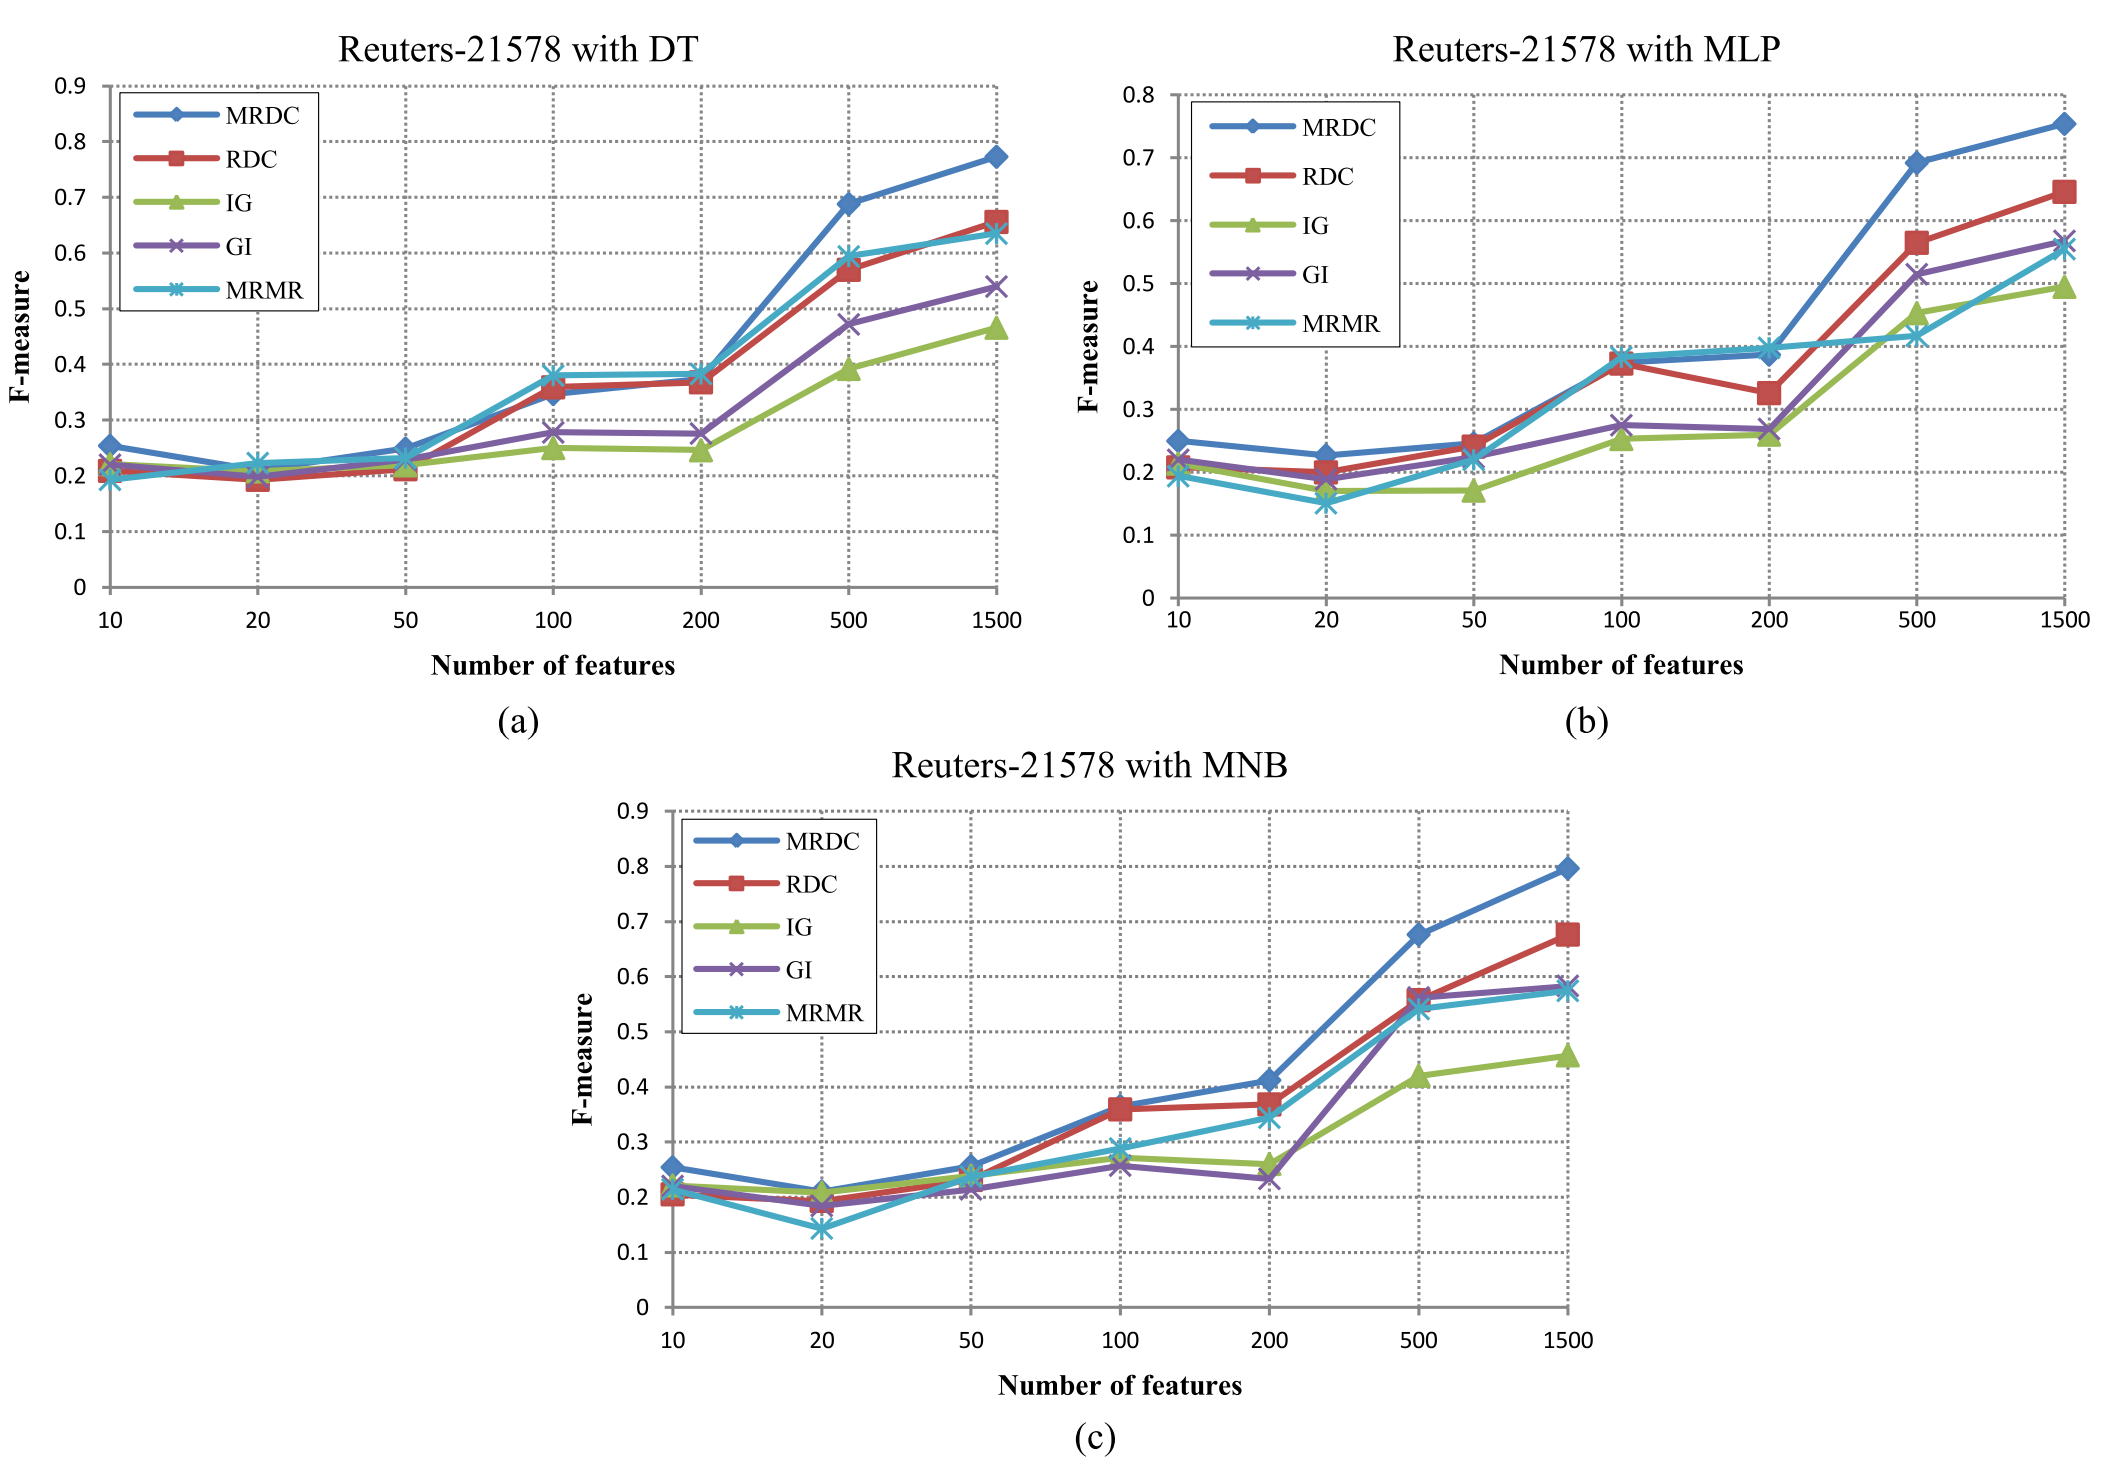
\includegraphics[height=11cm]{MRDC1.png}
\caption{امتیاز معیار $F_1$ برای روش‌های مختلف انتخاب ویژگی و روش \lr{MDRC} برای دسته‌بندی‌های مختلف \cite{labani2018novel} }
\end{figure}

\subsection{دقت روش برپایه الگوریتم ژنتیک}
در تصویر ۴-۳ برای یکی از مجموعه‌داده‌های مورد بررسی مقاله غارب و همکاران و برای دسته‌بندی \lr{Naive Bayes} کارایی دسته‌بندی قبل و بعد از اعمال الگوریتم برپایه ژنتیک ارائه‌شده بر شش روش پایه انتخاب ویژگی نشان داده شده است. در این جدول همچنین تعداد کاهش ویژگی هم نشان داده شده است. در این جدول می‌توان دید برای روشی مانند \lr{CDM} با وجود کاهش تعداد ویژگی، دقت بهبود یافته است که این نشان می‌دهد خروجی روش پایه شامل تعدادی ویژگی زائد است. برای روشی مانند بهره اطلاعاتی دقت ثابت مانده است اما تعداد ویژگی‌ها کاهش چشمگیری داشته است به طوری که برای حالت هزار ویژگی حدود هفتاد درصد کاهش رخ داده است. در کل به نظر می‌رسد استفاده از این الگوریتم برای کاهش ویژگی‌ها بعد از یک الگوریتم کاهش ویژگی کلاسیک ارزشمند باشد؛ چراکه هم منجر به کاهش تعداد ویژگی‌ و هم منجر به بهبود دقت می‌شود.
\\

سوال دیگری که پیش می‌آید این است که «آیا دقت این روش بهتر است یا روش \lr{MDRC} ؟» در این مورد واقعا نمی‌توان به صورت قطعی نظر داد. چراکه مجموعه‌داده‌ها و تنظیمات کاملا متفاوت است.

\begin{figure}[!h]
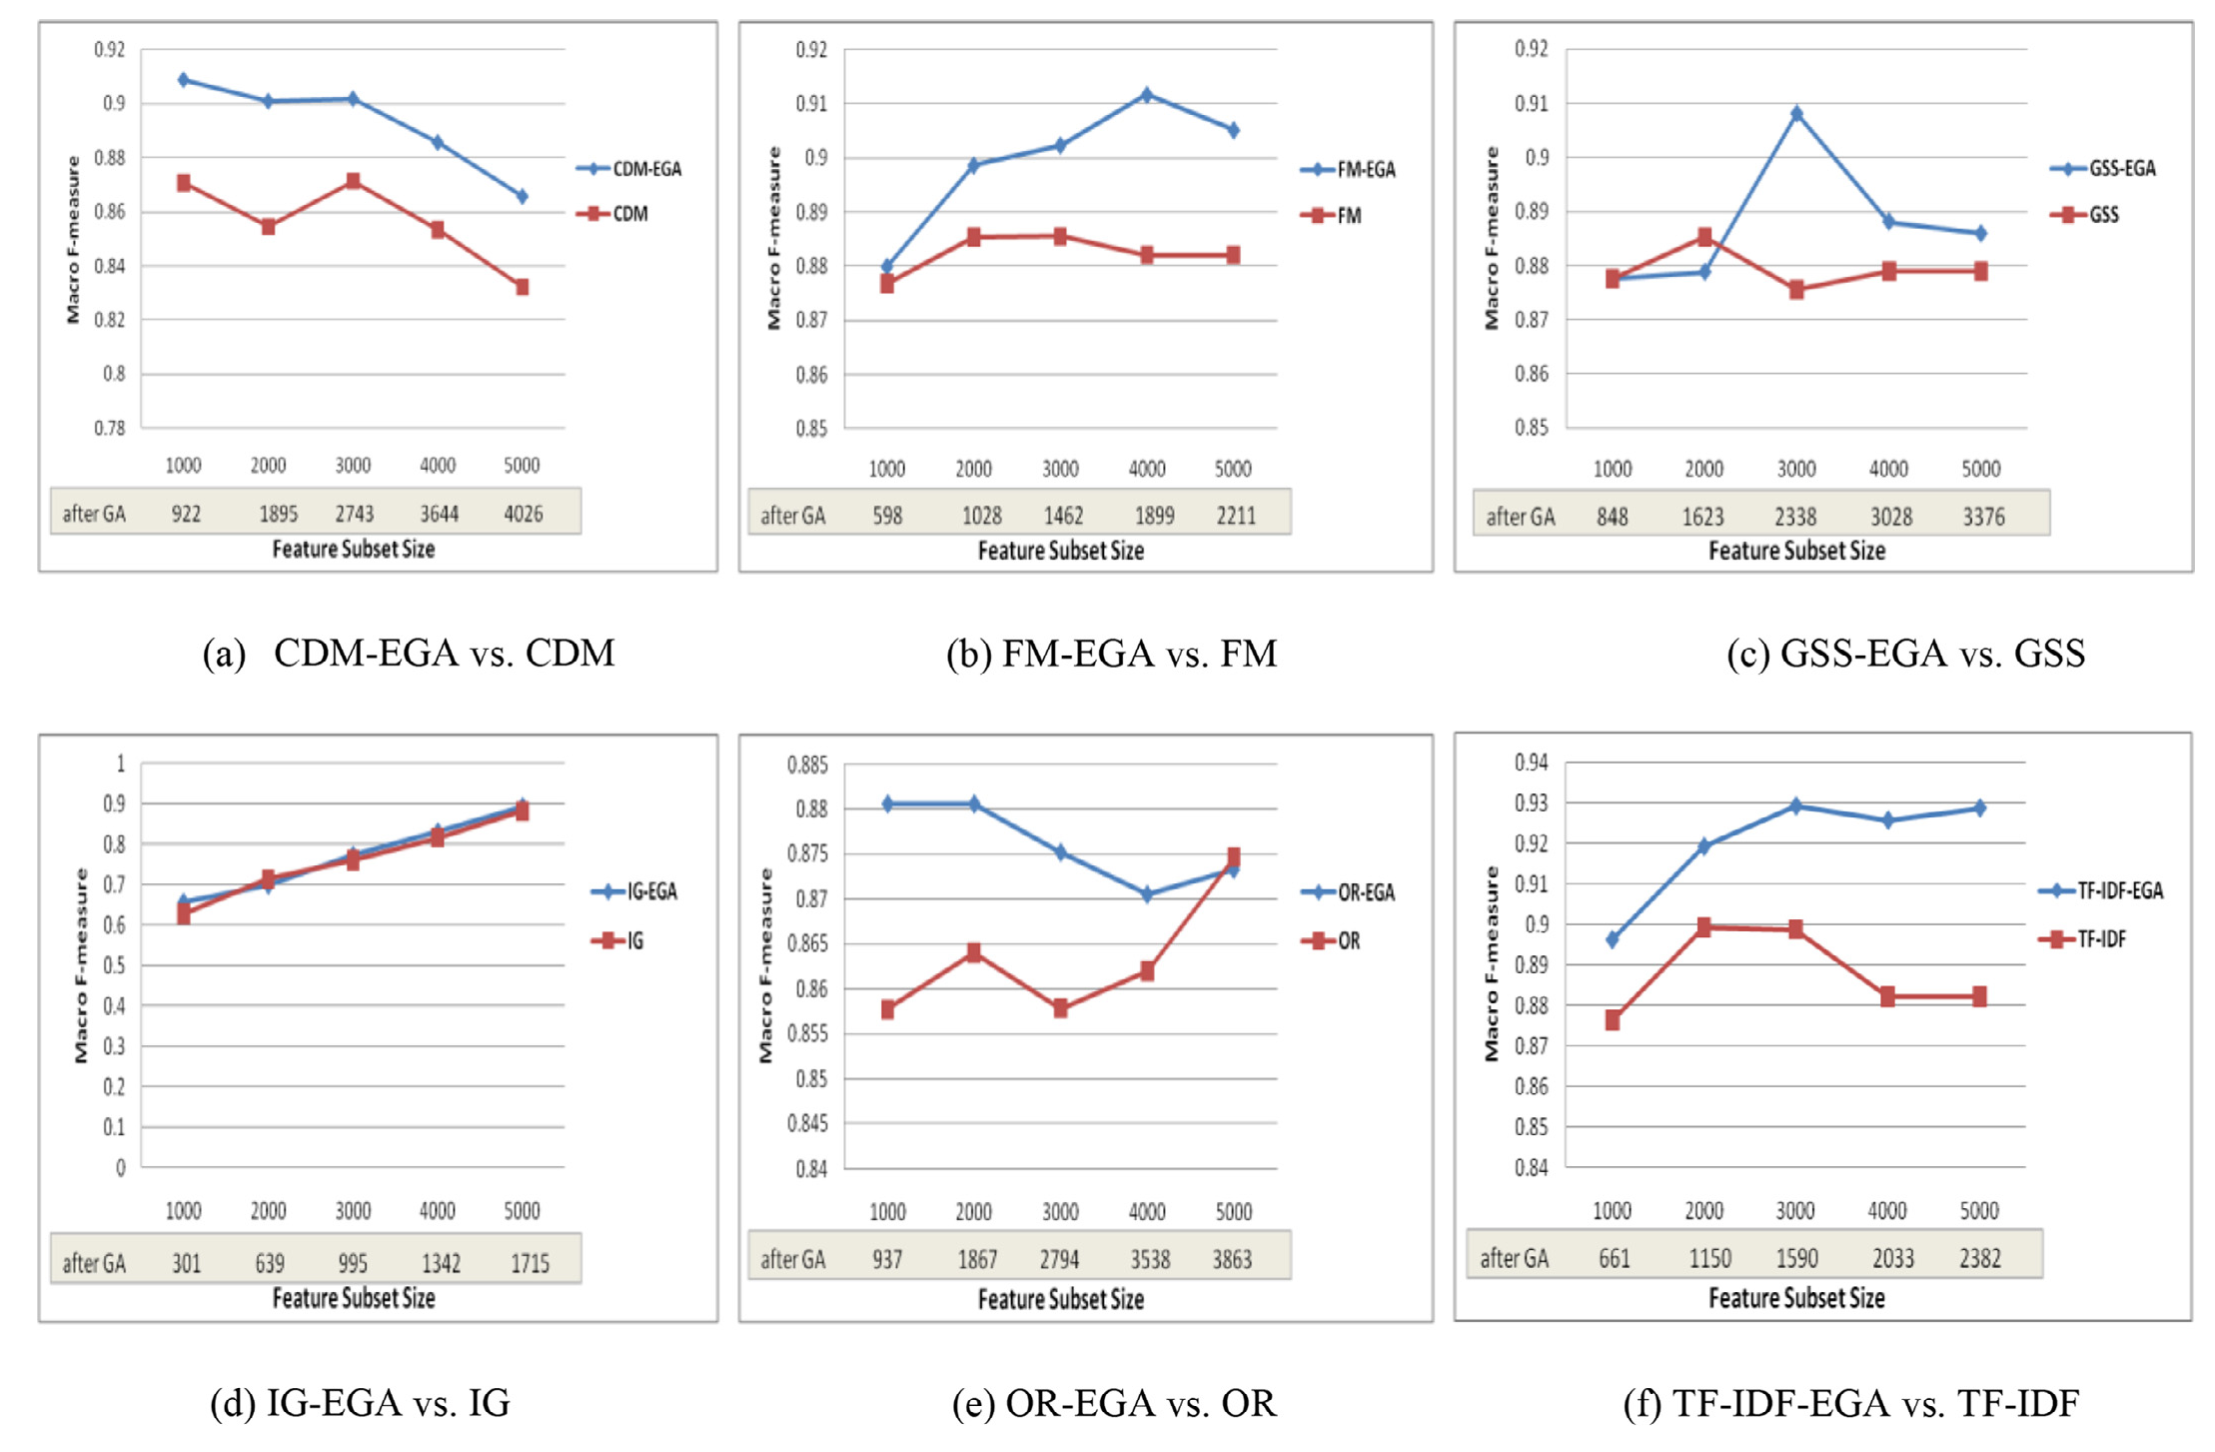
\includegraphics[height=11cm]{EGA1.png}
\caption{امتیاز معیار $F_1$ و همچنین کاهش تعداد ویژگی‌ها بعد از اعمال روش برپایه ژنتیک بر روش‌های پایه \cite{ghareb2016hybrid} }
\end{figure}

\section{مقایسه نوآوری}
یکی دیگر از شاخصه‌هایی که می‌توان روش‌های ارائه شده را با یکدیگر مقایسه کرد بحث نوآوری و ایده‌ای است که پشت روش‌های وجود داشته است. در این میان به نظر من روش برپایه ژنتیک خلاقانه‌تر بوده است. اگرچه این روش نخستین روشی نبوده است که بر روی الگوریتم ژنتیک در حوزه دسته‌بندی متن کار کرده است\cite{ghareb2016hybrid}، اما ایده‌های مربوط به بازترکیب و جهش آن مناسب بوده است. روش \lr{MDRC} کمترین نوآوری را داشته است؛ چراکه کل ایده روش بر پایه این موضوع است که برای انتخاب هر ویژگی، ویژگی‌ای را مدنظر قرار داد که با سایر ویژگی‌های انتخاب‌شده همبستگی پایینی داشته باشد. نهایتا روش \lr{IGFSS} را من در رتبه میانی از این منظر قرار می‌دهم.

\section{جمع‌بندی مقایسه‌ها}
در مجموع مواردی که مطرح شد، روش \lr{IGFSS} بهترین زمان اجرا را دارد و پس از آن روش \lr{MDRC} قرار دارد. اما روش \lr{MDRC} توانسته است دقت بهتری را بدست بیاورد. هرچند خلاقیت روش \lr{IGFSS} بیشتر بوده است. روش برپایه ژنتیک از هر دو روش حافظه و زمان اجرای بدتری دارد اما می‌توان نوآوری و ایده‌های خلاقانه بیشتری در آن دید. 